\documentclass{beamer}

\usepackage[utf8]{inputenc}
\usepackage[frenchb]{babel}
\usepackage{verbatim}
\usepackage{graphicx}
\usepackage{color}
\usepackage{hyperref}
\usepackage{verbatim}
\usepackage{url}
\usepackage{moreverb}
\usepackage{fancyvrb}
\usepackage{minted}
\usepackage{algpseudocode}
\usepackage{natbib}
\usepackage{eulervm}
\usepackage{auto-pst-pdf}
\usepackage{pst-plot}


\hypersetup{colorlinks=true, linkcolor=black, urlcolor=blue}
\usetheme{boxes}
\beamertemplatenavigationsymbolsempty
\setbeamertemplate{sections/subsections in toc}[circle]
\setbeamertemplate{footline}[frame number]
\setbeamertemplate{itemize items}[circle]
\setbeamertemplate{itemize subitem}[square]

\title{{\bf Understanding Random Forests}\\
From Theory to Practice}
\author{Gilles Louppe}
\institute{Université de Liège, Belgium}
\date{October 9, 2014}

\newcommand{\todo}[1]{\textcolor{red}{[TODO] #1}}

\definecolor{lightgreen}{rgb}{0.0,0.8,0.0}
\definecolor{lightblue}{rgb}{0.3,0.8,1.0}
\definecolor{lightred}{rgb}{0.874,0.180,0.105}
\definecolor{gray}{rgb}{0.4,0.4,0.4}
\definecolor{lightgray}{rgb}{0.8,0.8,0.8}
\definecolor{shadecolor}{rgb}{0.9,0.9,0.9}
\newrgbcolor{mygreen}{.00 .5 .00}
\newrgbcolor{myyellow}{.6 .6 .00}

\DeclareMathOperator*{\argmax}{arg\,max}


\newrgbcolor{mygreen}{.00 .5 .00}
\newcommand{\X}[1]{\textcolor{blue}{#1}}
\newcommand{\y}[1]{\textcolor{red}{#1}}
\newcommand{\model}[1]{\textcolor{mygreen}{#1}}
\newcommand{\loss}[1]{\textcolor{lightblue}{#1}}

\begin{document}

% Title page ==================================================================

\begin{frame}
\titlepage
\end{frame}


% Motivation ==================================================================

\begin{frame}
  \frametitle{Outline}
  \tableofcontents
\end{frame}

\section{Motivation}

\begin{frame}{Motivation}

\begin{figure}
\vspace{-0.5cm}
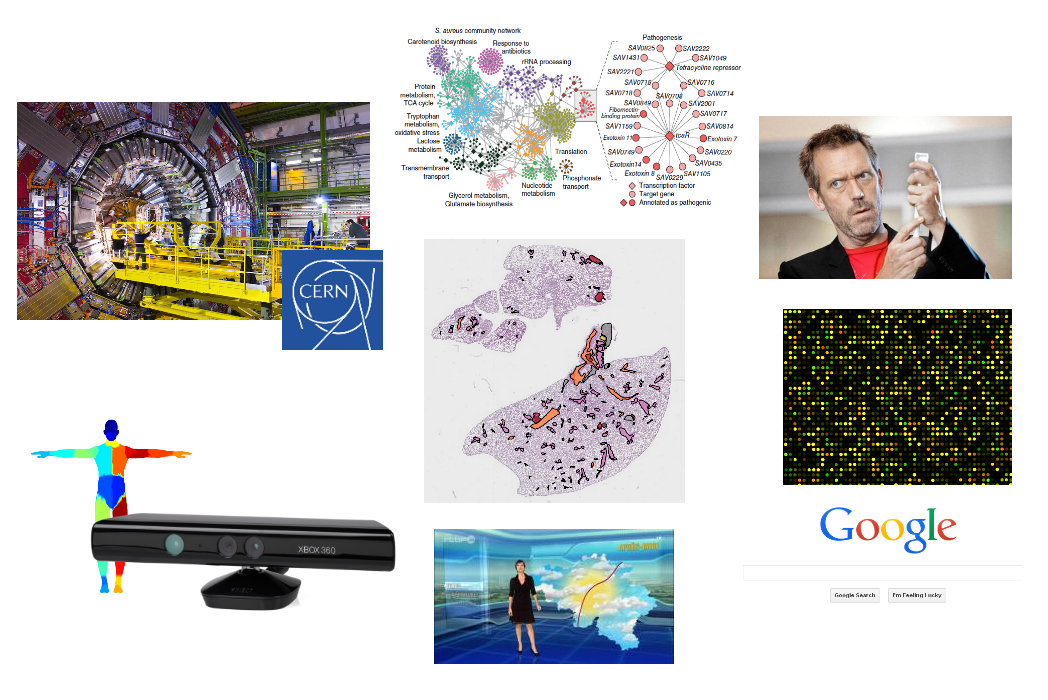
\includegraphics[scale=0.4]{./figures/motivation.png}
\end{figure}

\end{frame}

\begin{frame}{Objective}

\begin{center}
From a set of {\bf \X{measurements}},

\vspace{1cm}
learn a {\bf \model{model}}
\vspace{1cm}

to predict and understand {\bf \y{a phenomenon}}.
\end{center}

\end{frame}

\begin{frame}{Running example}

\begin{columns}
\begin{column}{0.5\textwidth}

\begin{center}
From {\bf \X{physicochemical properties}} (alcohol, acidity, sulphates, ...),

\vspace{1cm}
learn a {\bf \model{model}}
\vspace{1cm}

to predict {\bf \y{wine taste preferences}} (from 0 to 10).

\end{center}

\end{column}
\begin{column}{0.5\textwidth}
  \begin{figure}
  \vspace{-0.5cm}
  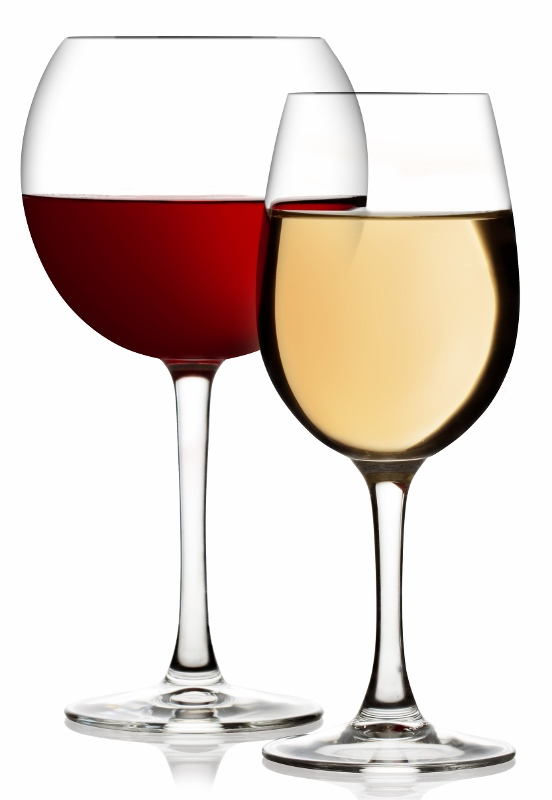
\includegraphics[scale=0.6]{./figures/wine.jpg}
  \end{figure}
\end{column}
\end{columns}

\vspace{1cm}

{\footnotesize
P. Cortez, A. Cerdeira, F. Almeida, T. Matos and J. Reis,
{\it Modeling wine preferences by data mining from physicochemical properties},
2009.}

\end{frame}


% Supervised learning =========================================================

\AtBeginSection[]
{
\begin{frame}
  \frametitle{Outline}
  \tableofcontents[currentsection]
  % Die Option [pausesections]
\end{frame}
}

\section{Growing decision trees}

\begin{frame}{Supervised learning}

\begin{itemize}
\item The \X{inputs} are random variables \X{$X = X_1$, ..., $X_p$};
\item The \y{output} is a random variable \y{$Y$}.
\end{itemize}

\begin{itemize}
\item Data comes as a finite learning set $${\cal L} = \{(\X{\mathbf{x}_i}, \y{y_i}) | i = 0, \dots, N-1 \},$$
where \X{$\mathbf{x}_i \in {\cal X} = {\cal X}_1 \times ... \times {\cal X}_p$} and \y{$y_i \in {\cal Y}$}
are randomly drawn from $P_{\X{X},\y{Y}}$.\\
\vspace{0.3cm}
E.g., $(\X{\mathbf{x}_i}, \y{y_i}) = ((\X{\text{color}=\text{red}}, \X{\text{alcohol}=12}, ...), \y{\text{score}=6})$
\end{itemize}

\begin{itemize}
\item The goal is to find a model $\model{\varphi_{\cal L}}: \X{{\cal X}} \mapsto \y{{\cal Y}}$ minimizing
$$
Err(\model{\varphi_{\cal L}}) = \mathbb{E}_{\X{X}, \y{Y}}\{ L(\y{Y}, \model{\varphi_{\cal L}}(\X{X})) \}.
$$
\end{itemize}

\end{frame}

\begin{frame}{Performance evaluation}

\begin{itemize}

\item {\it Classification} (e.g. ${\cal Y} = \{ \text{yes}, \text{no} \}$):
  $$L(Y, \varphi_{\cal L}(X)) = 1(Y \neq \varphi_{\cal L}(X))$$
  {\it \footnotesize (Number of times the predictions are wrong.)}

\vspace{1cm}

\item {\it Regression} (e.g. ${\cal Y} = \mathbb{R}$):
  $$L(Y, \varphi_{\cal L}(X)) = (Y - \varphi_{\cal L}(X))^2$$
  {\it \footnotesize (Large errors are more penalized.)}

\end{itemize}

\end{frame}


% Decision trees ==============================================================

\begin{frame}{Divide and conquer}
\begin{figure}
\only<1>{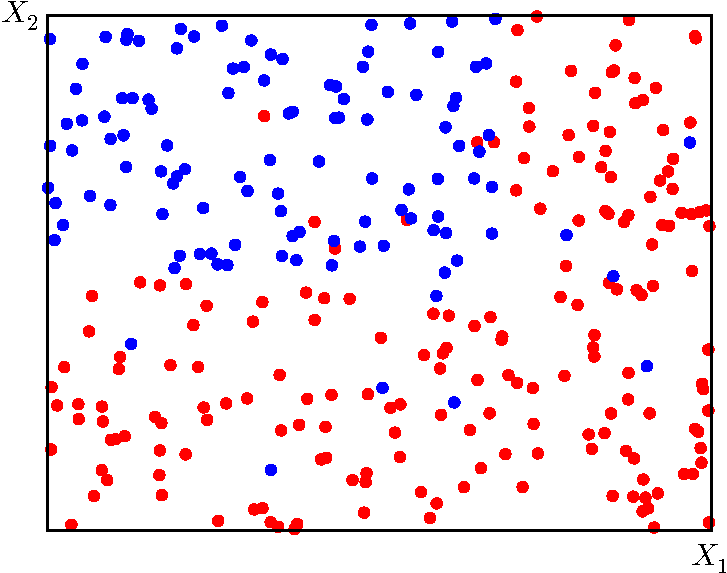
\includegraphics[scale=0.75]{./figures/tree-partition-c.pdf}}
\only<2>{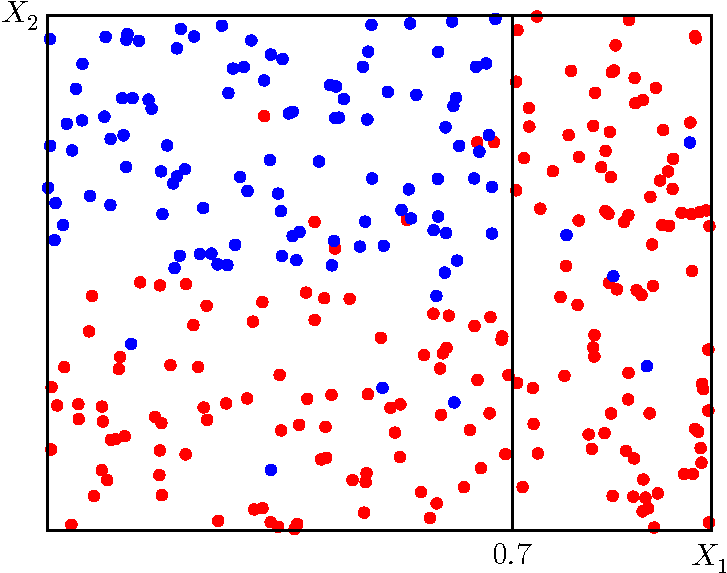
\includegraphics[scale=0.75]{./figures/tree-partition-b.pdf}}
\only<3>{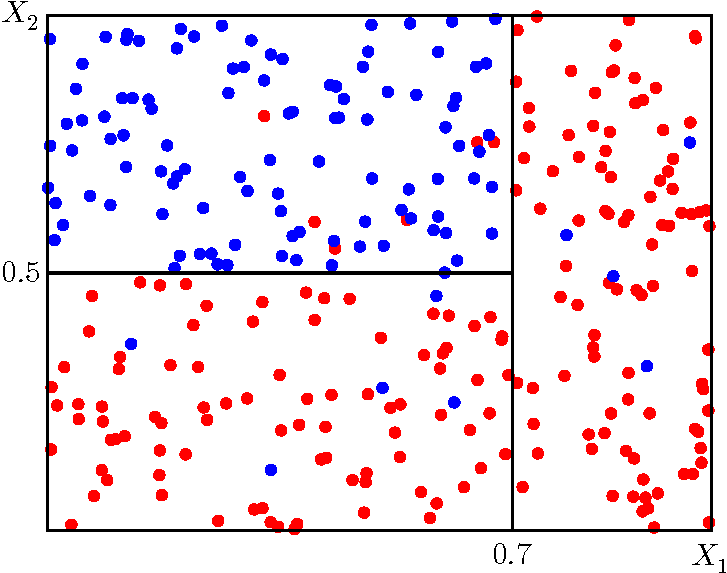
\includegraphics[scale=0.75]{./figures/tree-partition-a.pdf}}
\end{figure}
\end{frame}

\begin{frame}{Decision trees}
\begin{figure}
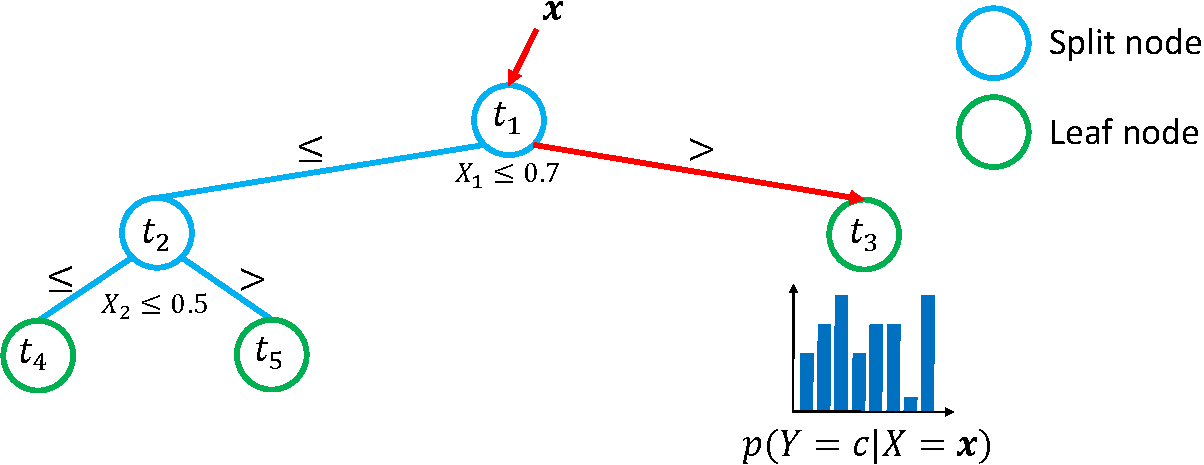
\includegraphics[scale=0.5]{./figures/tree-simple.pdf}
\end{figure}

$t \in \varphi$: nodes of the tree $\varphi$\\
$X_t$: split variable at $t$ \\
$v_t \in \mathbb{R}$: split threshold at $t$\\
$\varphi(\mathbf{x}) = \argmax_{c \in {\cal Y}} p(Y = c | X = \mathbf{x})$
\end{frame}

\begin{frame}{Back to our example}
\begin{figure}
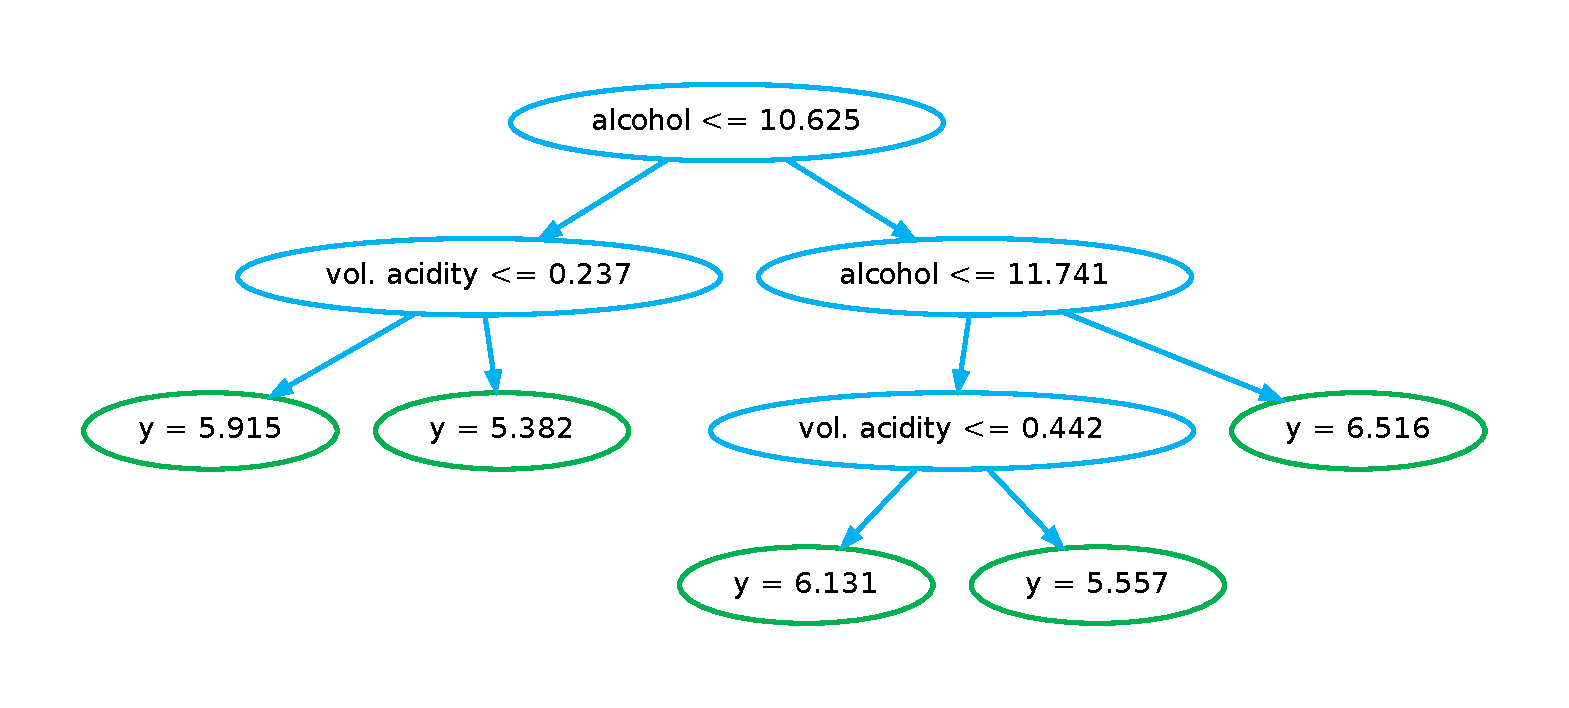
\includegraphics[scale=0.4]{./figures/tree-wine.pdf}
\end{figure}
\end{frame}

% Bias-variance ===============================================================

\begin{frame}{Bias-variance decomposition}

\begin{columns}
\begin{column}{0.65\textwidth}

{\bf Theorem.} For the squared error loss, the bias-variance decomposition of the expected
generalization error at $X=\mathbf{x}$ is
\begin{equation*}
\mathbb{E}_{\cal L} \{ Err(\varphi_{\cal L}(\mathbf{x})) \} = \text{noise}(\mathbf{x}) + \text{bias}^2(\mathbf{x}) + \text{var}(\mathbf{x})
\end{equation*}
where
\begin{align*}
\text{noise}(\mathbf{x}) &= Err(\varphi_B(\mathbf{x})), \\
\text{bias}^2(\mathbf{x}) &= (\varphi_B(\mathbf{x}) - \mathbb{E}_{\cal L} \{ \varphi_{\cal L}(\mathbf{x}) \} )^2, \\
\text{var}(\mathbf{x}) &= \mathbb{E}_{\cal L} \{ (\mathbb{E}_{\cal L} \{ \varphi_{\cal L}(\mathbf{x}) \} - \varphi_{\cal L}(\mathbf{x}))^2 \}.
\end{align*}

\end{column}
\begin{column}{0.35\textwidth}

\begin{figure}
\vspace{-1cm}
\hspace*{-0.4cm}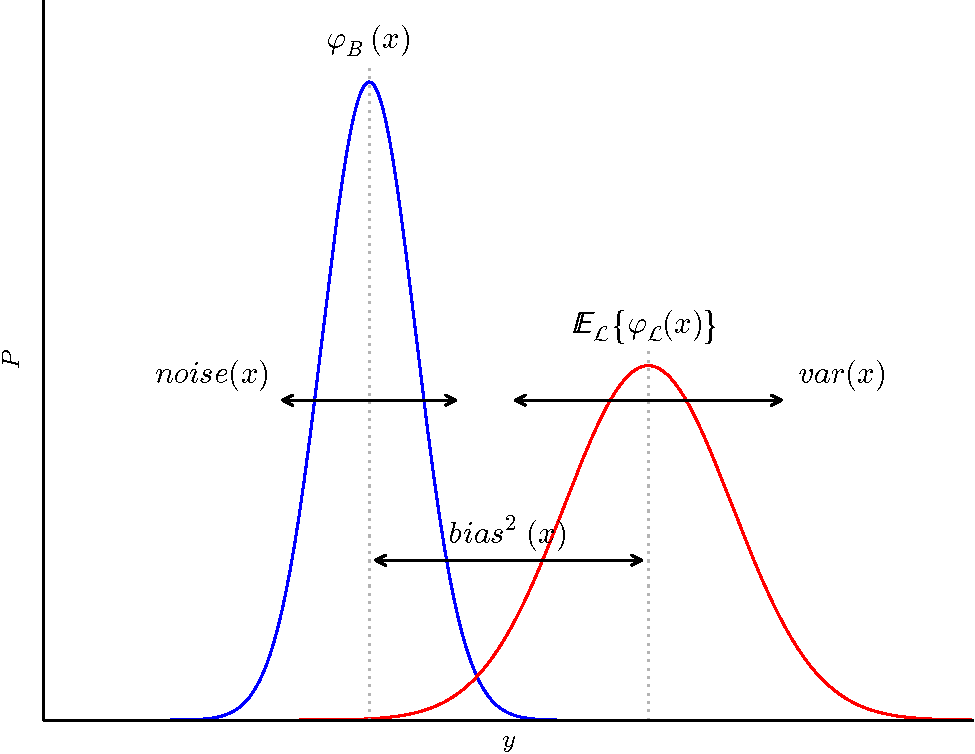
\includegraphics[scale=0.3]{./figures/bias-variance.pdf}\\
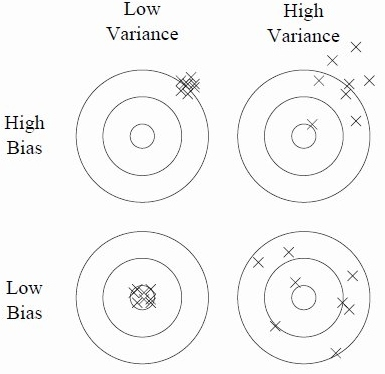
\includegraphics[scale=0.4]{./figures/bias-variance-darts.jpg}
\end{figure}

\end{column}
\end{columns}

\end{frame}

\begin{frame}{Diagnosing the generalization error of a decision tree}

\begin{itemize}
\item Residual error: Lowest achievable error, independent of $\varphi_{\cal L}$.
\item Bias: Decision trees usually have {\color{blue} low bias}.
\item Variance: They often suffer from {\color{red} high variance}.
\end{itemize}

\begin{itemize}
\item Solution: {\it Combine the predictions of several randomized trees into a single model.}
\end{itemize}

\end{frame}


% Forests =====================================================================

\begin{frame}{Random forests}
\begin{figure}
    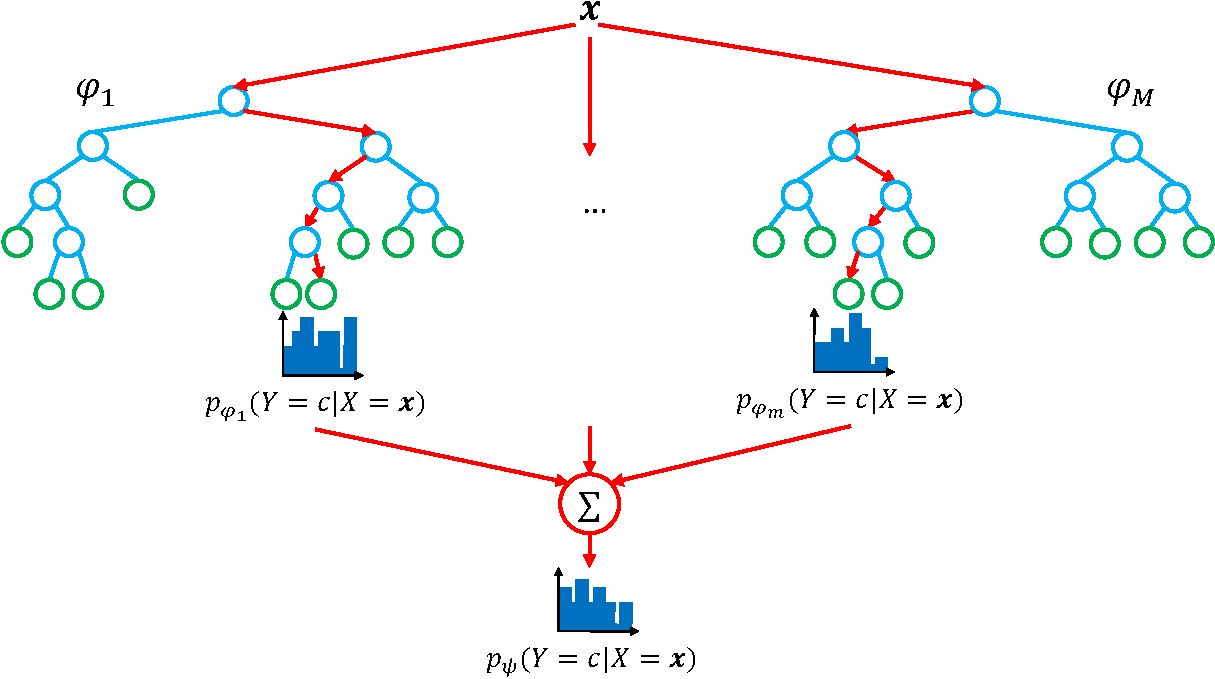
\includegraphics[scale=0.5]{./figures/forest.pdf}
\end{figure}

Ensemble of $M$ randomized decision trees $\varphi_m$\\
$\psi(\mathbf{x}) = \argmax_{c \in {\cal Y}} \frac{1}{M} \sum_{m=1}^M p_{\varphi_m}(Y = c | X = \mathbf{x})$
\end{frame}

\begin{frame}{Condorcet's jury theorem}

\begin{columns}
\begin{column}{0.65\textwidth}
Let consider a group of $M$ voters.

\vspace{1cm}

If each voter has an independent  probability $p > \tfrac{1}{2}$ of voting for
the correct decision, then adding more voters increases the probability of the
majority decision to be correct.

\vspace{1cm}

When $M \to \infty$, the probability that the
decision taken by the group is correct approaches $1$.

\end{column}

\begin{column}{0.35\textwidth}
\begin{figure}
    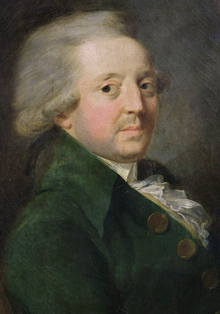
\includegraphics[scale=1.0]{./figures/condorcet.png}
\end{figure}
\end{column}
\end{columns}

\end{frame}


\begin{frame}{Bias-variance decomposition (cont.)}

{\bf Theorem.}
For the squared error loss, the bias-variance decomposition of the expected
generalization error $\mathbb{E}_{\cal L} \{ Err( \psi_{{\cal L},\theta_1,\dots,\theta_M}(\mathbf{x}))
\}$ at $X=\mathbf{x}$ of an ensemble of $M$ randomized models $\varphi_{{\cal L},\theta_m}$ is
\begin{equation*}
\mathbb{E}_{\cal L} \{ Err(\psi_{{\cal L},\theta_1,\dots,\theta_M}(\mathbf{x})) \} = \text{noise}(\mathbf{x}) + \text{bias}^2(\mathbf{x}) + \text{var}(\mathbf{x}),
\end{equation*}
where
\begin{align*}
\text{noise}(\mathbf{x}) &= Err(\varphi_B(\mathbf{x})), \\
\text{bias}^2(\mathbf{x}) &= (\varphi_B(\mathbf{x}) - \mathbb{E}_{{\cal L},\theta} \{ \varphi_{{\cal L},\theta}(\mathbf{x}) \} )^2, \\
\text{var}(\mathbf{x}) &= \rho(\mathbf{x}) \sigma^2_{{\cal L},\theta}(\mathbf{x}) + \frac{1 - \rho(\mathbf{x})}{M} \sigma^2_{{\cal L},\theta}(\mathbf{x}).
\end{align*}

and where $\rho(\mathbf{x})$ is the Pearson correlation coefficient between
the predictions of two randomized trees built on the same learning set.

\end{frame}

\begin{frame}{Interpretation of $\rho(\mathbf{x})$}

{\bf Theorem.} $\rho(\mathbf{x}) = \frac{\mathbb{V}_{\cal L} \{ \mathbb{E}_{\theta|{\cal L}} \{ \varphi_{{\cal L},\theta}(\mathbf{x}) \} \}}{\mathbb{V}_{\cal L} \{ \mathbb{E}_{\theta|{\cal L}} \{ \varphi_{{\cal L},\theta}(\mathbf{x}) \} \} + \mathbb{E}_{\cal L} \{ \mathbb{V}_{\theta|{\cal L}} \{ \varphi_{{\cal L},\theta}(\mathbf{x}) \} \}}$

\vspace{1cm}

In other words, it is the ratio between
\begin{itemize}
\item the variance due to the learning set and
\item the total variance, accounting for random effects due to both the
  learning set and the random perburbations.
\end{itemize}

\begin{itemize}
\item $\rho(\mathbf{x}) \to 1$ when variance is mostly due to the learning set;
\item $\rho(\mathbf{x}) \to 0$ when variance is mostly due to the random perturbations.
\end{itemize}

\end{frame}

\begin{frame}{Diagnosing the generalization error of random forests}

\begin{itemize}
\item Residual error: Lowest achievable error, independent of $\psi_{\cal L}$.
\item Bias: {\color{blue} Identical} to the bias of a single randomized tree.
\item Variance: As $M \to \infty$, {\color{red} $\text{var}(\mathbf{x}) \to \rho(\mathbf{x}) \sigma^2_{{\cal L},\theta}(\mathbf{x})$}
  \begin{itemize}
    \item The stronger the randomization, $\rho(\mathbf{x}) \to 0$, $\text{var}(\mathbf{x}) \to 0$.
    \item The weaker the randomization, $\rho(\mathbf{x}) \to 1$, $\text{var}(\mathbf{x}) \to \sigma^2_{{\cal L},\theta}(\mathbf{x})$
  \end{itemize}
\end{itemize}

\vspace{1cm}

{\bf Bias-variance trade-off.} Randomization increases bias but makes it
possible to reduce the variance of the corresponding ensemble model. The crux
of the problem is to {\color{red} find the right trade-off}.

\end{frame}

\begin{frame}{Back to our example}

\begin{table}
    \centering
    \begin{tabular}{| l c c |}
    \hline
        \textit{Method} & \textit{Trees} & \textit{MSE}  \\
    \hline
    \hline
    CART & 1 & 1.055 \\
    Random Forest & 50 & 0.517 \\
    Extra-Trees & 50 & 0.507 \\
    \hline
    \end{tabular}
\end{table}

\vspace{0.5cm}

\begin{center}
Combining several randomized trees indeed works better!
\end{center}

\end{frame}

\begin{frame}{Strengths and weaknesses of random forests}

\begin{itemize}
\item Very good accuracy
\item Universal approximation
\item Robustness to outliers
\item Robustness to irrelevant attributes (to some extent)
\item Invariance to scaling of inputs
\item Good computational efficiency and scalability

\bigskip

\item<2> \alert{Loss of interpretability with respect to single decision trees}
\end{itemize}

\end{frame}


% Bias-variance ===============================================================

\section{Interpreting random forests}


\begin{frame}{Variable importances}

\begin{itemize}
\item Interpretability can be recovered through {\color{blue}variable importances}

\bigskip

\item Two main importance measures:
    \begin{itemize}
    \item {\bf The mean decrease of impurity (MDI)}: summing total impurity reductions
      at all tree nodes where the variable appears {\scriptsize (Breiman et al., 1984)};
    \item {\bf The mean decrease of accuracy (MDA)}: measuring
      accuracy reduction on out-of-bag samples when the values of the
      variable are randomly permuted {\scriptsize (Breiman, 2001)}.
    \end{itemize}

\bigskip

\item We focus here on MDI because:
\begin{itemize}
\item It is faster to compute;
\item It does not require to use bootstrap sampling;
\item In practice, it correlates well with the MDA
  measure (except in specific conditions).
\end{itemize}

\end{itemize}
\end{frame}

\begin{frame}{Mean decrease of impurity}

\begin{figure}
    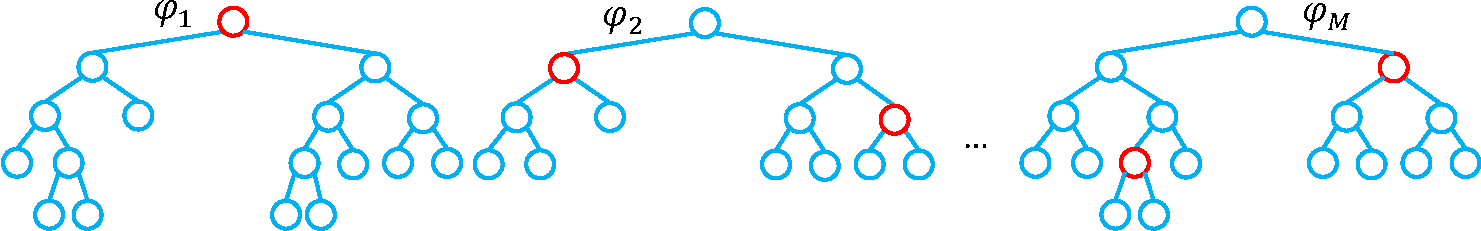
\includegraphics[scale=0.4]{./figures/mdi.pdf}
\end{figure}

Importance of variable $X_j$ for an ensemble of $M$ trees $\varphi_{m}$ is:
\begin{equation*}
\text{Imp}(X_j) = \frac{1}{M} \sum_{m=1}^M \sum_{t \in \varphi_{m}} 1(j_t = j) \Big[ p(t) \Delta i(t) \Big],
\end{equation*}
where $j_t$ denotes the variable used at node $t$, $p(t)=N_t/N$ and $\Delta i(t)$ is the impurity reduction at node $t$:
\begin{equation*}
\Delta i(t) = i(t) - \frac{N_{t_L}}{N_t} i(t_L) - \frac{N_{t_r}}{N_t} i(t_R)
\end{equation*}

\end{frame}

\begin{frame}{Back to our example}

MDI scores as computed from a forest of 1000 fully developed trees on the  Wine
dataset (Random Forest, default parameters).

\begin{figure}
    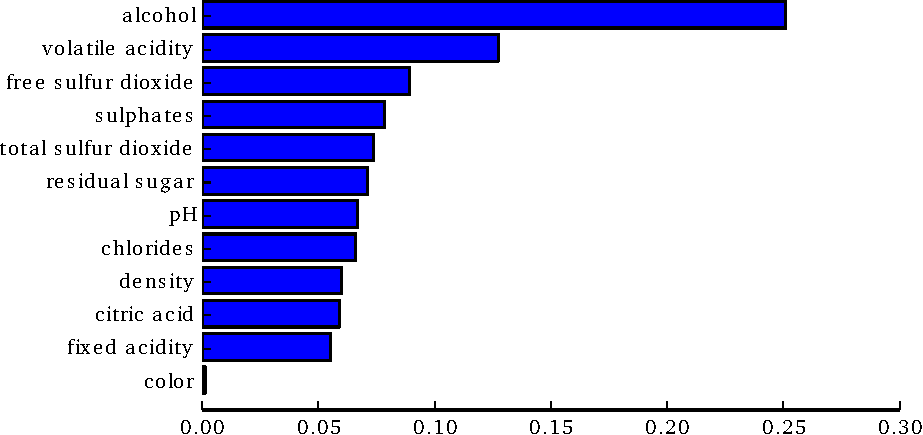
\includegraphics[scale=0.7]{./figures/imp-wine.pdf}
\end{figure}

\end{frame}

\begin{frame}{What does it mean?}
\begin{itemize}
\item MDI works well, but it is not well understood theoretically;
\item We would like to better characterize it and derive its main
  properties from this characterization.

\bigskip

\item Working assumptions:
\begin{itemize}
\item All variables are discrete;
\item Multi-way splits \`a la C4.5 (i.e., one branch per value);
\item Shannon entropy as impurity measure:
$$i(t) = - \sum_{c} \frac{N_{t,c}}{N_t} \log \frac{N_{t,c}}{N_t}$$
\item {\color{red} Totally randomized trees (RF with $K=1$);}
\item {\color{red} Asymptotic conditions: $N\to \infty$, $M\to \infty$.}
\end{itemize}
\end{itemize}
\end{frame}


\begin{frame}{Result 1: Three-level decomposition}

\hspace*{0.5cm}

{\bf Theorem.} Variable importances provide a three-level decomposition of the
information jointly provided by all the input variables about the output,
accounting for all interaction terms in a fair and exhaustive way.

\vspace{-0.5cm}

\begin{flalign*}
\underbrace{I(X_{1}, \ldots, X_{p} ; Y)}_{\substack{\text{Information jointly provided}\\
                                                                   \text{by all input variables}\\
                                                                   \text{about the output}}} =
\underbrace{\sum_{j=1}^{p}\text{Imp}(X_j)}_{\color{mygreen}\substack{\text{i) Decomposition in terms of}\\
                                                    \text{the MDI importance of}\\
                                                    \text{each input variable}}}\\
\end{flalign*}

\vspace{-1.5cm}

\begin{flalign*}
\text{Imp}(X_j) = \underbrace{\sum_{k=0}^{p-1} \frac{1}{C_p^k} \frac{1}{p-k}}_{{\color{blue} \substack{\text{ii) Decomposition along}\\
                                                                                                 \text{the degrees $k$ of interaction}\\
                                                                                                 \text{with the other variables}}}}
       \underbrace{\sum_{B \in {\cal P}_k(V^{-j})} I(X_j;Y|B)}_{{\color{red} \substack{\text{iii) Decomposition along all}\\
                                                                                            \text{interaction terms $B$}\\
                                                                                            \text{of a given degree $k$}}}}\\
\end{flalign*}

\vspace{-1cm}

{\scriptsize E.g.:~$p=3, \text{Imp}(X_1) = \frac{1}{3} I(X_1;Y)+\frac{1}{6}(I(X_1;Y|X_2)+I(X_1;Y|X_3))+ \frac{1}{3} I(X_1;Y|X_2,X_3)$}

\end{frame}

\begin{frame}{Illustration: 7-segment display {\scriptsize (Breiman et al., 1984)}}

\only<1>{
\begin{columns}
\begin{column}{0.3\textwidth}
\begin{figure}
    \vspace{-0.5cm}
    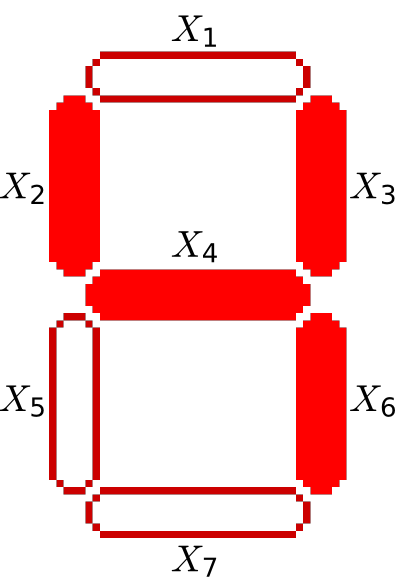
\includegraphics[scale=0.35]{./figures/led-fig.png}
\end{figure}
\end{column}
\begin{column}{0.7\textwidth}
\begin{center}
    \begin{tabular}{| c | c c c c c c c |}
    \hline
    $y$ & $x_1$ & $x_2$ & $x_3$ & $x_4$ & $x_5$ & $x_6$ & $x_7$ \\
    \hline
    \hline
    0 & 1 & 1 & 1 & 0 & 1 & 1 & 1 \\
    1 & 0 & 0 & 1 & 0 & 0 & 1 & 0 \\
    2 & 1 & 0 & 1 & 1 & 1 & 0 & 1 \\
    3 & 1 & 0 & 1 & 1 & 0 & 1 & 1 \\
    4 & 0 & 1 & 1 & 1 & 0 & 1 & 0 \\
    5 & 1 & 1 & 0 & 1 & 0 & 1 & 1 \\
    6 & 1 & 1 & 0 & 1 & 1 & 1 & 1 \\
    7 & 1 & 0 & 1 & 0 & 0 & 1 & 0 \\
    8 & 1 & 1 & 1 & 1 & 1 & 1 & 1 \\
    9 & 1 & 1 & 1 & 1 & 0 & 1 & 1 \\
    \hline
    \end{tabular}
\end{center}
\end{column}
\end{columns}
}

\only<2>{
\begin{equation*}
\text{Imp}(X_j)=\sum_{k=0}^{p-1} \frac{1}{C_p^k} \frac{1}{p-k} \sum_{B \in {\cal P}_k(V^{-j})} I(X_j;Y|B)
\end{equation*}
  \begin{columns}[t]
\begin{column}{0.3\textwidth}
\begin{center}
    \begin{tabular}{| c | c |}
    \hline
        Var & Imp \\
    \hline
    \hline
    $X_1$ & 0.412 \\
    $X_2$ & 0.581 \\
    $X_3$ & 0.531 \\
    $X_4$ & 0.542 \\
    $X_5$ & 0.656 \\
    $X_6$ & 0.225 \\
    $X_7$ & 0.372 \\
    \hline
    \hline
    $\sum$& 3.321 \\
    \hline
    \end{tabular}
\end{center}
\end{column}
\begin{column}{0.7\textwidth}
\begin{center}
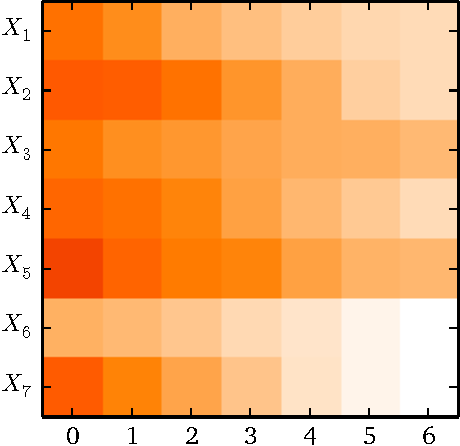
\includegraphics[width=0.7\textwidth]{figures/led-imp.pdf}\\
\hspace{0.5cm}$k$
\end{center}
\end{column}
\end{columns}
}

\end{frame}

\begin{frame}{Result 2: Irrelevant variables}

{\bf Theorem.} Variable importances depend only on the relevant variables.

\vspace{1cm}

\textbf{Definition} {\scriptsize (Kohavi \& John, 1997)}. A variable $X$ is
{\it irrelevant} (to $Y$ with respect to $V$) if, for all $B\subseteq V$,
$I(X;Y|B)=0$. A variable is {\it relevant} if it is not irrelevant.

\vspace{1cm}

{\bf Theorem.} A variable $X_j$ is irrelevant if and only if $\text{Imp}(X_j)= 0$.

\vspace{1cm}

{\color{blue} $\Rightarrow$ The importance of a relevant variable is
insensitive  to the addition or the removal of irrelevant variables.}

\end{frame}

\begin{frame}{Bias due to masking effects}

Most properties are lost as soon as $K>1$.

\bigskip

{\color{blue}$\Rightarrow$ There can be relevant variables with zero
importances (due to masking effects).}

\medskip

{\footnotesize
Example:\\
$I(X_1;Y)=H(Y)$, $I(X_1;Y) \approx I(X_2;Y)$, $I(X_1;Y|X_2)=\epsilon$ and $I(X_2;Y|X_1)=0$
\begin{itemize}
\item $K=1 \rightarrow \text{Imp}_{K=1}(X_1) \approx \frac{1}{2} I(X_1;Y)+\epsilon$ and $\text{Imp}_{K=1}(X_1)\approx \frac{1}{2} I(X_2;Y)$
\item $K=2 \rightarrow \text{Imp}_{K=2}(X_1)=I(X_1;Y)$ and $\text{Imp}_{K=2}(X_2)=0$
\end{itemize}}

\bigskip

{\color{blue}$\Rightarrow$ The importance of relevant variables can be
influenced by the number of irrelevant variables.}

\medskip

{\footnotesize
\begin{itemize}
\item $K=2$ and we add a new irrelevant variable $X_3$ $\rightarrow$ $\text{Imp}_{K=2}(X_2)>0$
\end{itemize}}

\end{frame}

\begin{frame}{Bias due to empirical impurity misestimations}

For a finite learning set ${\cal L}$ of size $N$, node impurity terms $i(t)$
suffer from an empirical misestimation bias.

\bigskip

If $X_j$ and $Y$ are independent random variables, then the expected value of
the finite sample size estimates   is:

\begin{equation*}
\mathbb{E}\{ \widehat{I}(X_j; Y) \} = \frac{(|{\cal X}_j|-1)(|{\cal Y}|-1)}{2 N_t \log 2}.
\end{equation*}

{\color{blue}$\Rightarrow$ Importances are biased towards variables of  high
cardinality.}

\medskip

{\color{blue}$\Rightarrow$ This effect can be minimized by collecting impurity
terms measured from large enough sample only (e.g., by stopping the
construction of the tree early).}

\end{frame}

\begin{frame}{Bias due to binary trees and threshold selection}

Random forests usually make use of binary splits instead of multiway exhaustive
splits.

\bigskip

{\color{blue}$\Rightarrow$ $i(t)$ does not actually measure the mutual
information.}

\bigskip

{\color{blue}$\Rightarrow$ Caution should be taken when interpreting the
numerical  value of importance scores.}

\end{frame}

\begin{frame}{Back to our example}

MDI scores as computed from a forest of 1000 fixed-depth trees on the  Wine
dataset (Extra-Trees, $K=1$, $\texttt{max\_depth}=5$).

\begin{figure}
    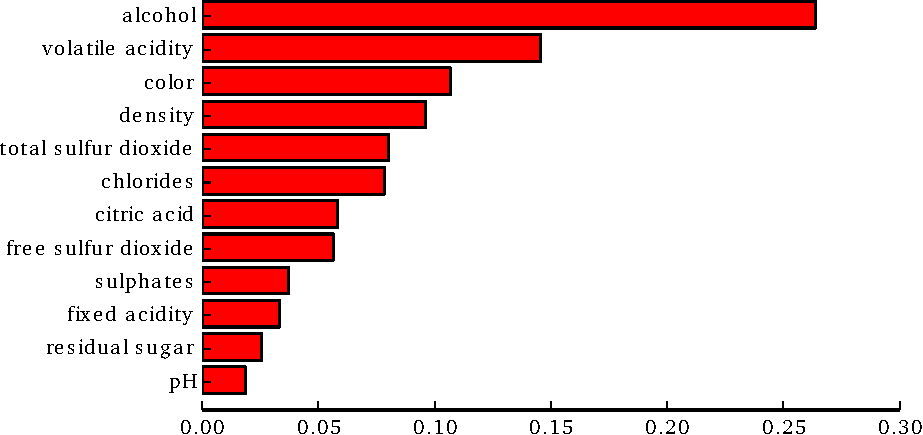
\includegraphics[scale=0.7]{./figures/imp-wine2.pdf}
\end{figure}

\begin{center}
Taking into account (some of) the biases results in a different story!
\end{center}

\end{frame}


% Computational performance ===================================================

\section{Computational performance}

\begin{frame}{Complexity}
\end{frame}

\begin{frame}{Implementation}
\end{frame}

\begin{frame}{Random patches}
\end{frame}


% Conclusions =================================================================

\section{Conclusions}

\begin{frame}{Conclusions}
\end{frame}

\end{document}
